\renewcommand\thechapter{c2.4}
\lab{The electric potential}\label{lab:electric-field}

\section*{About this lab}

\covid\ 
It is intended to be used during the fourth week in Physics 222.
It does not assume any previous knowledge of capacitors or
capacitance, so it can be used as soon as students know about
Gauss's law, electric field lines, and the electric potential
(Young and Freedman ch.~23, or Fields and Circuits ch.~4).

\apparatus
\equip{1.5 V battery}
\equip{battery holder}
\equip{multimeter}
\equip{replacement fuses for multimeter}
\equip{banana-plug cables (made by the student)}
\equip{capacitors (bipolar electrolytic, 50-330 $\mu\zu{F}$)}

\begin{goals}

\item[] Construct a capacitive voltage divider.

\item[] Test whether the electric field is nonconservative.

\end{goals}

\section*{To build before lab}
\makebanana

\introduction

\subsection*{A voltage divider}

Little kids easily manipulate magnetic fields using fridge magnets,
but electric fields are harder to control and do experiments on.
You can generate a static electric charge by scuffing your feet on
a carpet or rubbing a balloon on your hair, but this doesn't lend itself
to quantitative experiments, especially because the charge tends to
leak off while you're trying to do the measurement. Let's think about
what we would need to do in order to do something where we could really
measure something. We have three facts of life to deal with: (1) charge
can leak off; (2) what we can measure easily with a meter is the
potential $\phi$, not the field $\vc{E}$, although the two are closely
related; (3) we need to be able to deposit charge on objects in a controlled way.

Because objects like hair and balloons are electrical insulators,
charge can stick on them in a clumpy way, like a kindergartener's
fingerpaints. For better control and reproducibility, we want to use
an electrical conductor such as a metal. The first figure shows a realistic
computer simulation of what happens if we release a finite number of
charges onto a pear-shaped conductor. Because the charges  repel each
other, they all end up on the surface. The distribution of charge is
not uniform, but it is not random, either. With realistic numbers of
charges, the equilibrium charge distribution is completely reproducible,
and in this equilibrium arrangement the potential is constant throughout
the entire conductor.

\fig{em-fie-covid-pear}

To get the charge on there in the first place, we need at least two
conductors, which we can connect to the terminals of a battery.
The battery is a device that (ideally) maintains a well-defined
difference in potential between its terminals, and this leads to
something like the idea shown below. The pear has a deficit of
electrons and the tube an excess. Electric field lines run from
the positive charges (nuclei of atoms that have lost some electrons)
to the negative ones.

\fig{em-fie-covid-two-conductors}

This is all fine except that with only two objects, there is nothing
of any interest to measure. We can only measure a difference in potential,
using a voltmeter, and the voltmeter's two probes have to be connected
to a conductor --- the device doesn't work if we just wave the probes
in the air. In the experiment with two objects,
all we have is one object at the potential of
the battery's positive terminal and another at the potential of its
negative terminal. If the battery is, say, 1.5 volts, then the only
numbers we'll ever get are $+1.5$, 0, or $-1.5$ volts. So we will
need to have at least three conductors.

Finally, we have the issue of charge leaking off. In the setup shown
above, the pear and tube would both hold an extremely tiny amount of
charge, perhaps a picocoulomb. They would probably hold this charge just fine until
we touched them with the probes of the meter, but then this tiny quantity of charge would
flow back through the voltmeter in a fraction of a second. An ideal
voltmeter would be a perfect electrical insulator, but real-life ones
are not perfectly insulating.

For this reason, we need to use a device that holds a much larger amount
of charge than the Dr.~Seuss setup shown above. Such a device is called
a capacitor, and although the setup above is a capacitor, it's a capacitor
that doesn't store very much charge when we put a certain potential difference
across it.

The simplest capacitor to understand is a pair of parallel
metal plates with air or a vacuum between them. The detailed
physics of capacitance, its units of measurement, and so on, are topics
for later in this course, but the figure below shows the general idea.

\fig{em-fie-covid-capacitor-params}\label{fig:em-fie-covid-capacitor-params}

If you count all the pieces of metal in the figure, you'll see that there are three,
which is the minimum number, for the reasons described earlier.
In this example we compare two capacitors that are similar
except that the size of the plates is doubled in the bottom one. In order to make this
a fair comparison, we connect up the two capacitors in series (end to end) and
hook up the battery (not shown) externally between the very top and
very bottom. To see how this makes for a fair comparison, look at the
isolated island of metal in the middle, which is shaped sort of like
a capital ``I.'' This metal is surrounded by insulation such as air,
so no charge can get in or out of it. It starts with zero total charge,
so it will always have zero total charge. For this reason we are
guaranteed to have equal amounts of charge on the top of
the wide capacitor ($+6$ units) and the bottom of the narrow one ($-6$ units).
(These charges also attract other, opposite charges from the outside world onto
the outward-facing plates, so that the total charge on each capacitor is
zero.)

If we now compare the electric field lines that run from the positive
charges to the negative ones, we see that both capacitors contain 6 field
lines, but in the wider capacitor they are spaced twice as far apart.
Since the electric field lines in the narrow capacitor are twice as dense,
its internal electric field is twice as strong. If the capacitors were
like rooms with gravitational fields in them, you would feel twice as
heavy inside the narrow room, and gravitational potential energies
inside that room would be doubled. In electrical terms, the thing we
can actually measure is the electric potential $\phi$, which is the
electric potential energy per unit charge. If you measured the potential
difference across each of these capacitors using a voltmeter, you would
find that even though you gave them each a fair chance and put the same
amount of charge on it, the bottom one would display half as much of a potential
difference.

Summarizing these ideas, we say that every capacitor has a certain numerical
rating called its capacitance, $C$, in units called farads (F), which we will
define more formally later in the course. In the example above, the wide
capacitor has twice the capacitance, and therefore it ends up with half as much potential difference across it. The capacitors you will 
use in this lab are not actually parallel-plate capacitors with vacuum
between the plates, but that doesn't matter for our purposes. They can
still be given ratings in units of farads, and for the series circuit we're using
we have the inverse proportionality $\Delta\phi\propto 1/C$, as in the visual example.

You will notice that the capacitors we use in this lab are fairly big
and bulky, about the size of your thumb. The reason they're so physically
big is that we need to use big capacitances in order to get a lot of charge and keep the charge
from leaking off quickly when we take measurements. The ones in this lab are in the range of tens or hundreds
of microfarads. ``Micro-'' may sound small, but it's actually a pretty
big value for a capacitance. Most of the capacitors in a typical piece
of electronics are in the nano- or picofarad range. For
the capacitance values we use in this lab, the leaking off of charge through the meter will take place on time scales of a few
minutes, so there is no problem with taking a measurement fast enough
and then disconnecting the probes.\footnote{We'll go into the mathematical
details later, but in case you're interested, the leakage time goes like
the product $RC$, where $R$ is the resistance of the voltmeter and $C$ is
the capacitance. The meter we're using does have a pretty big resistance,
about a million ohms, but for example if we used a one-microfarad
capacitor, the leakage time would be only one second.}

\fig{em-fie-europe}

\subsection*{Conservative and nonconservative fields}

The figure above shows a map of part of Europe.\footnote{\url{commons.wikimedia.org/wiki/File:Blank_map_of_Europe_in_1920.svg},
CC-BY-SA license} Suppose you decide to walk all the way around the border of France,
eventually returning to your starting point. Newtonian gravity, which is an excellent approximation for the earth's
gravitational field, predicts that the gravitational field is conservative, so that along any such closed path,
the work done on you by the gravitational field is zero. In other words, any climbing you do on this hike will be canceled
out by the elevation losses from going downhill. If we break the route up into pieces, then for example the segment
from A and B will have a significant change in elevation, because B is near the crest of the Alps. Hiking from A to B
will be an elevation gain, whereas if you went the opposite way and hiked from B to A, the elevation gain would be
negative. Thus if you wanted to check that the total elevation gain on this loop was zero, you would need to decide
on a clockwise or counterclockwise orientation for your hike, and you would also need to make sure that when you
measured elevation differences, you defined their signs in a way that was consistent with this orientation.

In the second figure, we make the map into a circuit containing a bunch of capacitors and batteries. You will make
up a circuit for this lab that is like this but simpler, with only five components.
There are various loops we can trace in this circuit. There is one around the border of France, containing six circuit
elements, one around the border of Switzerland that has three, and so on. There are also other loops we could draw.
For instance, we could start from the west coast of France and ``hike'' clockwise around the outer perimeter of the whole
figure, which would take us through 9 components.

Both magnetic and electric fields can be either conservative or nonconservative.
A nonconservative field is ``swirly'' or ``curly,'' and may contain field lines
that form closed loops. These concepts are discussed in your text at greater length and
with more mathematical precision. Theory predicts that \emph{static} electric fields
like the ones in this lab should be conservative. Only for a conservative field does
it make sense to talk about a potential $\phi$, as we have been casually 
doing.\footnote{For a nonconservative field, what a voltmeter measures is actually the work
per unit charge needed to move a charge from point A to point B, through the meter, and this could
change, for example, if you wiggled the meter so that the path became different.}
For a conservative field, the sum of the voltage changes around a closed loop will be zero. 

It turns out that if we check only the \emph{inner} loops, i.e., the border of every country,
then no more information is obtained by checking other loops such as the big outer loop. If we write down the four equations
asserting that each inner loop adds up to zero, then it is possible to prove that every loop in the circuit adds up to
zero. Therefore for the purpose of this lab, it is only necessary to do all the inner loops of whatever circuit you create.

\observations

\setcounter{labpartctr}{0}

\labpart{A voltage divider}

Your kit includes four capacitors with values in the range from 50 to 330 $\mu\zu{F}$.
Pick two of these that are different in value but not by an order of magnitude.
Physically small capacitors have their values labeled on them in very brief and
not completely standardized ways, but for big ones like this there should simply
be some printed value that's easy to interpret.

Build the circuit shown in the diagram below. In this style of drawing, called
a schematic, we don't realistically show the shapes and sizes of the capacitors.
This is called a series circuit, meaning that it's a single loop like a necklace.

\fig{em-fie-covid-voltage-divider}

The symbol for the battery looks a little bit like the one for a capacitor, but
it's actually a completely different device.
The battery is a polar device, i.e., its two sides are different from each other.
The higher potential is indicated by the longer line.
Some capacitors are also polar, and need to be hooked up with the right polarity
or they will not work or explode. The capacitors in your kit are nonpolar ones,
so it doesn't matter which way you put them in. (Capacitors that are polar have
stripes or other marks to indicate which way they have to be used.)

The next figure, drawn in a mixture of schematic and realistic styles,
shows how to measure the potential difference created by the
battery. The details are drawn to resemble the meter I expect to send out with
your kit, but in any case multimeters are pretty standardized. Turn on the
meter by turning the rotary knob to the 2000 mV (2000 millivolt) scale, which reads in units of
volts and is capable of handling voltages up to two volts. If you connect the wires
as shown, you should get a positive reading. The nominally 1.5 V alkaline batteries
we're using are actually about 1.6 V.

\fig{em-fie-covid-voltage-divider-meter-1}

Note that a voltmeter is always connected to a circuit in parallel like this,
because it measures the difference in potential between the two points touched
by its probes. It isn't necessary to take apart the circuit in order to use
a voltmeter like this, and normally just touching the wires together is good
enough, although you can stick one banana plug into another if you like, for
a more solid connection.

Now reposition the probes of the meter to measure the potential difference
$\Delta\phi_1$ across $C_1$ and the difference $\Delta\phi_2$ across $C_2$.
You should find that, as in the  figure on p.~\pageref{fig:em-fie-covid-capacitor-params}, the potential
differences are unequal. Test whether they are in inverse proportion to the capacitances.

This type of capacitive voltage divider is sometimes used in real life when
one wants to use a meter to measure a large voltage. Imagine that instead of
1.5 volts, we had 1500 volts. Hooking up a meter to check this voltage directly would probably cause
the meter to explode in your face. But by using a voltage divider with two very
unequal capacitances, we could make a scaled-down copy of the voltage, which we
could then measure safely and interpret using an appropriate fudge factor determined from $C_1$ and $C_2$.
Usually this application is used for AC circuits, not a DC circuit
like the one in this lab, because of the leakage problems described above.

It is possible to unknowingly get bad data for the following reason. The analysis above
was predicated on the assumption that the ``island'' between the two capacitors would
always have zero total charge. Now consider the setup shown below, which is what you
would use to measure the voltage across one of the capacitors. The island is no longer
isolated from the rest of the universe. Charge can flow in or out of it through the
meter. If this starts to happen, then our analysis that proved $\Delta\phi \propto 1/C$ becomes
completely invalid. I tested this with the AstroAI meter and the two black capacitors
that came with the kit, and I found that after half an hour, the reading on the meter had
changed by 15\%. If I left it like this overnight, the capacitor would discharge completely
through the meter, and the reading would go to zero. This would not be a practical problem in 
this lab, since the leakage is fairly slow. 

\fig{em-fie-covid-voltage-divider-meter-discharge}

However, imagine that as you were fiddling
with your circuit, you inadvertently touched two of the wires together so that there was
a discharge path for the capacitor that was just some wire. This is called ``shorting across''
the capacitor. The discharging process would
be almost instantaneus. Your circuit would then be in a messed-up state, with nonzero total charge on the ``island,'' and you would
not necessarily have any idea of what was wrong. Similar problems can occur if you do things like
disassembling and reassembling your circuit, or swapping in a different capacitor. These high-value capacitors
can retain charge on their plates even when you toss them in a box overnight.

For these reasons, it's a good idea to carry out the following procedure to completely discharge
your capacitors before charging them up with the battery and taking data.
(1) Remove the battery from the holder. (2) Take two wires and use them to simultaneously
 short across the two capacitors, as in the figure below. (3) Remove the extra wires and then
put the battery back in the holder.
 After this process, the island is guaranteed to have zero
total charge in it.

\fig{em-fie-covid-voltage-divider-discharge}


\labpart{Constant potential on a conductor?}

In a one-piece object made of a perfect conductor, the potential should be constant everywhere.
The wires and alligator clips used in this lab are pretty good conductors (metals
such as copper and aluminum), but not perfect ones. For this reason, when we do
measurements like the ones in part A, we expect that it should
not matter too much if we choose to touch a probe of the voltmeter to one spot or another
on the same wire. But since these wires are pretty thin and made of real-world materials,
this may not be a perfect approximation. See if you can detect any voltage differences
between different parts of the same wire. 

Tips for making this a sensitive test: (1) Make the connections by shoving a banana plug into
the hole in another banana plug. Otherwise you may actually be measuring effects due to the
resistance of the connection itself. (2) Rather than repeating the measurements of
part A while varying the details of the connection, you can probably
get a more sensitive test by putting the meter on the 200 mV scale and using it to measure
the potential different between the connectors on the two ends of the same wire.

\labpart{Conservative, or nonconservative?}

Use all of your capacitors to build a more complicated version of part A.
To make this fun, don't make your circuit all parallel or all series. Make it some
combination of series and parallel parts. Make sure that all of your capacitors are
connected at both ends --- if they have one end dangling in the air, then that branch
is an open circuit, which might as well have not come to the party.

If you draw the schematic for this circuit, you should find that it's possible to lay it
out in such a way that no wires cross over other wires.\footnote{See \url{https://en.wikipedia.org/wiki/Planar_graph}.}
For each inner loop, use the meter to check whether the sum of voltage
drops around the loop is zero as predicted by theory.

As with the circuit from part A, this one has a possible state in which every ``island'' between capacitors
has zero total charge, as well as other possible states in which this is not true. In theory, this makes
no difference as to whether the field is conservative. However, it would be nicer to get the circuit into
a known state so that, for example, if you need to rebuild it later to get a missing piece of data, you can
do so. To do this, follow a procedure similar to the one used for discharging the capacitors in part A:
(1) take the battery out of the holder, (2) lay a piece of aluminum foil down on the circuit and put it
in electrical contact with every exposed contact at once, and (3) put the battery back in.

\section*{Preparation}

The figure on p.~\pageref{fig:terrier-conservative} shows a circuit
that contains only static electric fields.
Given the first two readings, we want to predict the third one.
Is it $+1$, $-1$, $+5$, or $-5$ V? Explain your answer.

Any of the four given possibilities can be obtained by adding the
voltages, depending on the signs. It matters how the voltmeter is
connected across each component (which side is COM and which is V),
and it also matters that one meter reading is positive and the other
negative. Without specifically discussing those details, there is no
way to determine which answer is correct.

\begin{figure*}
  \includegraphics{../figs/em-fie-terrier-conservative}\label{fig:terrier-conservative}
\end{figure*}

\analysis

For each part of the lab, compare theory with experiment, including error analysis.
Propagation of errors is described in appendix 3.
Give a probabilistic interpretation of the results, as in the examples at the end of appendix 2.

Common mistakes in part C: (1) Not considering the battery as a component.
(2) Treating the circuit as a whole rather than identifying loops. Most circuits
that students come up with contain two inner loops, each of which contains two to four
components.

For part A, the main source of error is the tolerances on
the capacitances.
The tolerances of the capacitors I intend to include in this kit are as
follows:
$330\ \mu\zu{F}\:\pm 20\%$,
$220\ \mu\zu{F}\:\pm 20\%$? (not stated, so this is a guess),
$68\ \mu\zu{F}\:\pm 10\%$,
$50\ \mu\zu{F}\:\pm 10\%$. 

For part C, it should be reasonable to estimate the error bars on the raw
data by using either the meter's maximum rounding error or the size of any visually
noticeable fluctuations in the reading, whichever is bigger.

